\documentclass[a4paper]{book}
%
% Sample journal layout stolen from IAnewsletter
% FOR ILLUSTRATION PURPOSES ONLY
% Do not reuse this format without permission from IATAC
%
\usepackage[left=16mm,right=0mm,textwidth=114mm,
     marginparwidth=69.5mm,includemp,top=35mm,
     bottom=20mm]{geometry}
\usepackage[utf8x]{inputenc}
\usepackage[T1]{fontenc}
\usepackage[svgnames]{xcolor}
\usepackage{fancyhdr,type1cm,lettrine,fix-cm,multicol,url,
     graphicx,mdwlist,fancybox,sectsty,bbding,calc,soul}
\usepackage{changepage}
%\usepackage{charter,avant}

\renewcommand{\thechapter}{}
\renewcommand{\thesection}{}

\definecolor{titlegrey}{cmyk}{.8,.8,.8,.2}
\renewcommand{\LettrineTextFont}{\normalfont}
\allsectionsfont{\sffamily}
\setcounter{secnumdepth}{0}
%
% One-page story makes its own heading block and sets the 
% leftmark for the running head
%
\newenvironment{story}[2][\relax]{%
  \if\relax#1\else
  \markboth{\MakeUppercase{#1}}\fi
  \vspace*{-6mm}\leavevmode\null\kern-21.5mm\fboxsep15mm%
    \colorbox{titlegrey}{\vbox to5mm{\hsize111mm\null\vfill
        \raggedright\color{white}\sffamily\huge\noindent
        \textbf{#2}\addcontentsline{toc}{chapter}{#2}\par\smallskip}}%
  \par\vspace{24pt}\parskip 7.2pt\raggedright
}{% end story
  }
%
% bulleting and indentation parameters for tagged lists
%
\setlength{\leftmargini}{14pt}
\setlength{\leftmarginii}{12pt}
\renewcommand{\labelitemi}{\rotatebox{90}{\scriptsize\TriangleDown}}
\renewcommand{\labelitemii}{\textbullet}
\makecompactlist{taglist}{itemize}
%
% parameters for adjusting height offset of top right image
% and the depth of the grey sidebar
%
\newlength{\vpicset}
\setlength{\vpicset}{68.75mm}
\newlength{\sbarheight}
\setlength{\sbarheight}{\textheight - \headheight - \vpicset}
% sidebar
\newenvironment{sidebar}[1]{%
  \begin{Sbox}\begin{minipage}{60mm}\raggedright
      \subsubsection*{#1}\parskip 7.2pt%
}{% end sidebar
  \end{minipage}\end{Sbox}\fboxsep5mm
  \marginpar{\null\vspace{0mm}\colorbox{LightGrey}{%
      \vbox to\sbarheight{\TheSbox\vfill}}}}
%
% push the image and running head into the headers
%
\pagestyle{fancy}
\fancyfoot[C]{}
\fancyfoot[L]{\small\sffamily\thepage\footnotesize\qquad
  \textbf{Manual do Ingressante} 2014\enspace\textbullet\enspace
  www.apogeeu.fee.unicamp.br}
\renewcommand{\headrulewidth}{0pt}

\newcommand{\CcImageBy}[1]{%
	\includegraphics[#1]{creative_commons/cc_by_30.pdf}%
}
\newcommand{\CcImageCc}[1]{%
	\includegraphics[#1]{creative_commons/cc_cc_30.pdf}%
}
\newcommand{\CcImageSa}[1]{%
	\includegraphics[#1]{creative_commons/cc_sa_30.pdf}%
}

%% Groups
\newcommand{\CcGroupBySa}[2]{% zoom, gap
	\CcImageBy{#1}\hspace*{#2}\CcImageSa{#1}%
}

\makeatletter
\renewcommand\tableofcontents{%
  %\pagestyle{plain}%
  \@starttoc{toc}}
\makeatother 

%%%%%%%%%%%%%%%%%%%%%%%%%%%%%%%%%%%%%%%%%%%%%%%%%%%%%%%%%%%%%%%%
\begin{document}

%%%%% Capa
%\thispagestyle{empty}

\changepage{+2cm}{+2cm}{-2cm}{-2cm}{}{-2cm}{}{}{}

\begin{figure}
    \voffset-2cm
	\includegraphics[scale=1.00]{frente.png}
	\label{fig:capa}
\end{figure}


%%%%% Licença
\input{licenca.tex}

\clearpage

\frontmatter

\begin{story}{Sumário}
\tableofcontents
\end{story}

\cleardoublepage

\mainmatter

%\renewcommand{\chaptername}{}
%\renewcommand{\thechapter}{}

%%%%% Boas vindas
% Este arquivo .tex será incluído no arquivo .tex principal. Não é preciso
% declarar nenhum cabeçalho

\setcounter{page}{1}

\begin{story}{Boas vindas}

Caro colega,

Parabéns, você acabou de ingressar em um dos poucos programas de pós-graduação em Engenharia Elétrica classificados pela CAPES como curso de excelência máxima (nota 7)! Em breve você irá perceber que não é apenas a estrutura e o nível do corpo docente que fazem uma pós-graduação desse nível, mas também a qualidade e dedicação dos seus alunos. Mas não se assuste! Apesar de todo o suor que você terá pela frente, você verá que ainda é possível conciliar trabalho firme nas aulas e na sua pesquisa com a vida social em Barão Geraldo e Campinas.

Este manual\footnote{Esse manual também pode ser encontrado em nossa página na internet, no endereço \url{www.apogeeu.fee.unicamp.br/manual-do-ingressante}.} foi organizado pela APOGEEU (Associação de Pós-Graduandos da Faculdade de Engenharia Elétrica e de Computação da Unicamp) com base no manual do Centro Acadêmico da Computação (CACo) -- \url{http://www.caco.ic.unicamp.br} --, escrito por diversos alunos que contribuíram com informações que serão especialmente úteis para você, ingressante! Assim, esperamos que vocês nos mandem informações sobre erros encontrados, informações sobre restaurantes novos ou que fecharam e por aí vai! Nosso e-mail é \url{apogeeu@fee.unicamp.br}.

Onde comer? Onde estudar? Onde morar? Tudo isso são dúvidas comuns, que aqui tentamos ajudar a resolver. Não há respostas prontas, cada um tem suas preferências, mas a gente dá uma mão.

O que é APG? E CPG? E CCPG? E RPG? Como eu faço para pegar uma bolsa? A gente também tenta responder todas essas perguntas. E também damos algumas dicas de onde comprar coisas, onde se divertir e alguns telefones úteis.

Já demos os parabéns, então agora vamos para o que importa: dar umas dicas para os seus primeiros passos na pós-graduação da Unicamp e apresentar a APOGEEU!

\section*{Mensagem do diretor da FEEC}
\addcontentsline{toc}{section}{Mensagem do diretor da FEEC}

Prezados pós-graduandos da FEEC,

É com grande satisfação que lhes damos boas-vindas à comunidade da Faculdade de Engenharia Elétrica e de Computação. Somos quase 100 docentes, quase 2000 estudantes, entre graduação e pós-graduação e cerca de 50 colaboradores que possibilitam o funcionamento de nossa escola. No orgulhamos de ser o melhor programa de pós-graduação em Engenharia Elétrica do Brasil, o que foi conseguido pelo mérito conjunto de nossos estudantes e professores.

A pós-graduação é mais um passo em um processo de educação que, mais do que nunca, tem que ser contínuo, permanente. O conhecimento é uma riqueza que não ocupa espaço, não tem massa, mas tem peso: o peso da responsabilidade. Estudar em uma escola pública, financiada com os impostos pagos pela sociedade paulista e brasileira, acresce ainda mais responsabilidade neste processo.

Os saberes de cada um estão em proporção direta com o que se pode esperar de sua atuação profissional, social, política. Assim, desejamos que a nova jornada que se inicia na vida de cada um de vocês lhes traga uma expansão de seus conhecimentos, seja em profundidade, seja em amplitude. Que se estabeleçam novas amizades e que estas perdurem no futuro. Que tenham uma atitude crítica perante nossa escola, o que nos permitirá melhorar continuamente, assim como ante o país e o mundo.

Daqui a algum tempo, terminada esta nova jornada, esperamos que as lembranças destes tempos que estão se iniciando sejam as melhores possíveis e que levar consigo um diploma da Unicamp seja um orgulho e um compromisso com um mundo melhor.

Bem-vindos à FEEC e à Unicamp!

\begin{flushright}
Prof. José Antenor Pomilio \\
Diretor da FEEC/Unicamp
\end{flushright}

\section*{Mensagem do coordenador de pós-graduação}
\addcontentsline{toc}{section}{Mensagem do coordenador de pós-graduação}

Prezado(a) aluno(a) ingressante,

Seja muito bem-vindo(a) ao Programa de Pós-Graduação em Engenharia Elétrica da Faculdade de Engenharia Elétrica e de Computação (FEEC) da UNICAMP! Você passa a fazer parte de um dos melhores programas de pós-graduação do país nesta área, que possui o conceito máximo (7) concedido pela CAPES, e que tem inserção importante tanto no cenário nacional como internacional.

Você inicia uma nova etapa de amadurecimento e aprendizado profissional, e muito lhe será exigido em termos de estudo, esforço, iniciativa, e disciplina. Naturalmente, a FEEC também se esforçará para lhe oferecer um ambiente de estudo de qualidade, com salas de aula e laboratórios adequados, e professores altamente qualificados, que lhe ajudarão a trilhar esse caminho árduo, porém, extremamente gratificante. Ao chegar ao final do caminho, você certamente sentirá a satisfação da vitória alcançada, o prazer de ter agregado novos conhecimentos à sua história de vida, e a segurança de um futuro promissor, ao longo do qual você poderá atuar de forma construtiva para o desenvolvimento da ciência e da sociedade.

É muito importante que, desde já, você comece essa caminhada com consciência e conhecimento dos seus direitos e deveres. Além da importância que você certamente dará aos seus estudos e pesquisas, deverá também atentar para as regras estabelecidas pelo programa. Você sabe quantos créditos em disciplinas deverá cursar? Sabe o que é o exame de qualificação e quais são os requisitos mínimos para realizá-lo? E o tempo de integralização? O que são as áreas de concentração? Como se convalida créditos? Quais são as condições mínimas para que você possa defender sua tese ou dissertação? As respostas a estas perguntas e a muitas outras mais você encontrará consultando o Catálogo dos Cursos de Pós-Graduação e a página da Comissão de Pós-Graduação (CPG) da FEEC, em

\begin{itemize}
\item \url{www.fee.unicamp.br/cpg}
\end{itemize}

No link Legislação, você terá acesso ao Regimento Geral dos Cursos de Pós-graduação da UNICAMP e ao Regulamento de Pós-graduação da FEEC. No link Alunos regulares você obterá as informações básicas sobre todos os requisitos para a obtenção do título almejado. O link Calendário lhe indica todas as datas importantes e as respectivas atividades. Há um link com perguntas frequentes (FAQ) e muito mais. Tudo isso para que você tenha segurança na sua caminhada, conhecendo as características e os prazos estabelecidos para cada uma de suas atividades. Aproveitamos para lembrar que na FEEC toda a regulamentação e prazos são seguidos de maneira rigorosa. Por isso, fique bem atento(a) e consulte a página da CPG com regularidade!

Ainda assim, se você tiver dúvidas, ou se simplesmente quiser conversar com a equipe da CPG, saiba que você será muito bem recebido(a) e nos esforçaremos para ajudá-lo(a) da melhor forma. É fundamental que você não tenha nenhum tipo de dúvida e não se veja em situação de prejuízo acadêmico por desconhecimento das regras e prazos. Conte conosco sempre!

Finalizo desejando-lhe muito sucesso!

\begin{flushright}
Prof. Carlos A. Castro \\
Coordenador de Pós-Graduação da FEEC/Unicamp
\end{flushright}

\end{story}


\cleardoublepage
%%%%% APOGEEU
% Este arquivo .tex será incluído no arquivo .tex principal. Não é preciso
% declarar nenhum cabeçalho

\begin{story}{A APOGEEU}

Antes de falar qualquer coisa, a primeira coisa que precisamos dizer é: \textbf{seja bem vindo à FEEC e parabéns por ter entrado na melhor faculdade de Engenharia Elétrica do país!}

Já que você já está aqui, não precisamos fazer propaganda das qualidades da nossa faculdade, do fato dela ser uma das raras instituições a ter nota 7 na CAPES (ou seja, nível de excelência internacional), da Unicamp ser a universidade mais bem avaliada pelo MEC, tanto na graduação quanto na pós-graduação, ou da nossa universidade ser responsável por cerca de 15\% da produção científica nacional.

Vamos aproveitar para falar aqui sobre a \textbf{APOGEEU}, a SUA associação de pós-graduandos a partir de agora!

Primeira pergunta: o que significa Associação de Pós-Graduandos (ou simplesmente APG)? Possivelmente quando você estava na graduação você tinha um centro acadêmico, que tinha como responsabilidade defender os alunos, representá-los junto à universidade, organizar atividades e outras coisas do tipo. Pois é, a APG tem essas funções também! A APOGEEU, por exemplo, organizou nos últimos tempos mini-cursos de estatística para experimentos, palestras, participou ativamente na reorganização do Programa de Estágio Docente da Unicamp e do estabelecimento de regras na faculdade para o acúmulo de bolsas de pós-graduação com outros rendimentos.

\section*{Trabalhar é preciso!}

A APOGEEU é atualmente uma das mais importantes associações de pós-graduandos do Brasil, de modo que tem tido papel fundamental na atual campanha pelo reajuste de bolsas de pós-graduação da CAPES e do CNPq, organizando manifestações e escrevendo artigos. Esse respeito adquirido é fruto de muito trabalho dos voluntários. Certamente poderia ser feito muito mais coisa, mas para isso é preciso de mais pessoas para trabalharem!

Nos últimos anos já realizamos muitas atividades, mas tínhamos planos de fazer muito mais! Queremos organizar cursos de redação científica, de línguas, de programação paralela em GPU e muitos outros. Queremos organizar mais palestras, mais discussões. Precisamos aumentar as ações pelo reajuste de bolsas (se continuarmos todos parados nada vai sair). Mas é claro, para isso precisamos de pessoas para ajudarem. Sem apoio não fazemos nada!

Então deixamos o convite para vocês todos participarem da APOGEEU, indo às nossas reuniões (que são realizadas todas as quartas, das 12h às 13h30) e/ou ajudando em atividades que interessem a vocês. Para ficarem informados sobre a APOGEEU, vocês podem se inscrever em nosso grupo de e-mails:

\begin{itemize}
\item \url{groups.google.com/group/apogeeu}
\end{itemize}

\section*{Oportunidades de crescimento pessoal}

Certamente que a parte principal de sua pós-graduação é no laboratório, mas tenha em mente que não é só isso e que há muitas outras formas de aprendizado que são importantes para você! Convênios de pesquisa, experiência de estágio docente, projetos de extensão universitária e atividades voluntárias também tem um papel importante na formação do professor/pesquisador que provavelmente você irá ser. A participação na associação de pós-graduandos e em atividades como representante discente junto à universidade são excelentes oportunidades para você fazer contatos importantes e aprender a ter um papel ativo onde quer que esteja, seja na academia, seja em uma empresa. Organização de eventos, discussões sobre a administração da universidade e maior conhecimento sobre as pesquisas desenvolvidas em outras partes da Unicamp são só alguns dos outros possíveis benefícios e que podem te dar um grande diferencial além de somente o título de mestre e doutor (que muitos outros no Brasil inteiro terão).

Assim, fica o incentivo a vocês buscarem outras atividades fora do seu mestrado/doutorado, para que o dinheiro que o cidadão do Estado de São Paulo investe em vocês possa valer muito mais! E fica também o convite para que essa atividade extra seja o trabalho junto à APOGEEU!

\section*{Onde encontrar a APOGEEU}

A sede da associação fica no prédio da pós graduação da FEEC, na sala PE27 (subindo um piso pelas escadas, entre no corredor à esquerda. Será a primeira porta à sua esquerda, antes dos armários). Para mais informações quanto à APOGEEU, incluindo o horário das reuniões e as normas para uso dos armários, visite o site:

\begin{itemize}
\item \url{www.apogeeu.fee.unicamp.br}
\end{itemize}

E, como somos modernos, temos Twitter -- \url{twitter.com/apogeeu} --, Facebook -- \url{facebook.com/APOGEEU} -- e Google+ -- \url{goo.gl/WQ9fO}. Precisando de qualquer coisa, você pode entrar em contato conosco pelo e-mail \url{apogeeu@fee.unicamp.br}.

\end{story}


\cleardoublepage
%%%%% Lugares para morar
% Este arquivo .tex será incluído no arquivo .tex principal. Não é preciso
% declarar nenhum cabeçalho

\begin{story}{Lugares para morar}

\begin{sidebar}{Moradia Estudantil} 

%\section*{Moradia Estudantil}
%\addcontentsline{toc}{section}{Moradia Estudantil}

A Moradia Estudantil (ou só ``Moradia'') é um conjunto de moradias contruído da Unicamp que são destinadas às pessoas que não teriam condições de se manter em Campinas pagando aluguel. A seleção para vagas na moradia é feita exclusivamente com base em critérios sociais. Para saber mais sobre o processo seletivo entre em:

\begin{itemize}
\item \url{www.sae.unicamp.br/portal/index.php?option=com_content&view=article&id=23&Itemid=155}
\end{itemize}

A moradia está localizada na Avenida Santa Isabel, 1125, a aproximadamente 3 km do campus da Unicamp. Cada casa (que normalmente é dividida entre quatro pessoas) se constitui de um quarto, uma cozinha, um banheiro e uma sala. Ainda tem o Circular da Moradia, um ônibus da Unicamp que transporta a galera durante o dia todo da moradia até a Unicamp e vice-versa.

\end{sidebar}

O preço de uma casa é a área do paralelepípedo formado pelos seguintes valores nos eixos: proximidade da Unicamp, tamanho da casa (quantidade de quartos) e qualidade da casa (acabamento, quantidade de banheiros etc). Quanto à distância, a avenida 1\footnote{Avenida 1 é o antigo nome da Avenida Dr. Romeu Tórtima, ainda muito usado.} e avenida 2\footnote{Assim como no caso da avenida 1, avenida 2 é o antigo nome da Avenida Prof. Atilio Martini.} são bem caras por serem próximas da Unicamp e as ruas entre elas muitas vezes também são. A região que vai do centro de Barão até a moradia, assim como a Cidade Universitária 2 (região próxima ao lago da Unicamp), geralmente são boas e barata para se morar: têm bastantes serviços e ainda são perto da Unicamp (mais ou menos 10 minutos de bicicleta). Se você tem carro, outras opções também são apartamentos no Jardim Santa Genebra (ao lado do Shopping Parque Dom Pedro) ou na Chácara Primavera (entre o shopping e o parque do Taquaral).

Além das dicas que se encontram a seguir nesse manual, você pode encontrar lugares para morar (especialmente repúblicas) no site Morar Unicamp:

\begin{itemize}
\item \url{morarunicamp.com.br}
\end{itemize}

\section*{Repúblicas}
\addcontentsline{toc}{section}{Repúblicas}

Geralmente a melhor escolha, se você tiver condições de pagar por uma moradia. Você pode levar quem quiser para sua casa (dependendo da aprovação dos moradores), chegar no horário que quiser, e conhecerá muita gente nova. Tente, se possível, morar em uma república de cursos mistos, pois assim você terá contatos diversos. O custo de uma vaga em uma república é muito variável (depende do nível de conforto que você quer). Em uma república ``normal'' o custo está em torno de R\$475,00 o aluguel para dividir quarto e R\$650,00 para pegar um quarto sozinho. Procure bem as pessoas com quem você vai morar para não ter problemas com diferentes estilos de vida (tem gente que gosta de lavar louça a cada 5 minutos e tem gente que gostaria de morar junto com porcos; veja com quem você se dá melhor).

Outra coisa importante é o tamanho da república. Repúblicas menores (3 a 5 pessoas) acabam dando mais certo, sendo mais organizadas e tendo melhores ambientes para estudar, mas saem mais caro do que morar com 13 pessoas (e existem repúblicas ainda maiores, acredite!). Veja o que mais se adapta a você e às suas posses financeiras. Para saber mais sobre repúblicas entre em:

\begin{itemize}
\item \url{www.republicasunicamp.com.br}
\end{itemize}

\section*{Quitinetes}
\addcontentsline{toc}{section}{Quitinetes}

Tomem cuidado com elas, pois a especulação imobiliária em Barão Geraldo chega a ser assustadora, e nos últimos anos ficou fora de controle. As quitinetes mobiliadas, normalmente um quarto-sala-cozinha-área de serviço e banheiro, estão com valores na ordem de R\$1000,00 ou mais. Sim, mais de mil reais por um micro espaço. Só porque é perto da Unicamp. Fique de olho e tome cuidado com os contratos.

As melhores relações custo-benefício de quitinetes são aquelas próximas ao centro de Barão Geraldo ou no espaço entre as avenidas. E lembre-se não é só de Unicamp que se vive. Não adianta pagar mais caro para estar do lado da Unicamp, se você fica muito longe dos mercados, farmácias etc.

\section*{Pensões}
\addcontentsline{toc}{section}{Pensões}

Dependendo da pensão que você conseguir pode tornar-se uma grande roubada. Algumas pensões não deixam você levar pessoas para sua casa, reclamam se você chegar tarde e não liberam festas, enquanto que outras não. Então procure bem! O preço também não é muito bom, mas às vezes é mais barato que quitinetes. É bom se você quer um esquema ``casa, comida e roupa lavada''. É muito importante que você saiba que contratos de um ano (ou qualquer período) em pensionatos são ilegais e você não precisa cumpri-los.

\section*{Dicas de segurança}
\addcontentsline{toc}{section}{Dicas de segurança}

Além de um novo ambiente de estudos, você conhecerá novos lugares e pessoas. E, provavelmente, em breve estará planejando sua mudança para Campinas. Muitos dos estudantes moram em Barão Geraldo, por ser mais perto da Unicamp, possibilitando que sua bicicleta se torne seu meio de transporte principal, por ser o lugar com maior número de repúblicas e pensionatos e por ser onde a maior parte das festas acontecem! No entanto, por ser constituído em sua maioria por casas de famílias com muitas posses e casas de estudantes (em geral desatentos), Barão Geraldo peca pela falta de segurança. Não é raro ouvir de alguma casa que foi saqueada durante um feriado prolongado. Portanto, é importante zelar pela sua integridade e de seus pertences - assim como sua família faz em sua casa, não importa onde ela more.

Se sua pensão ou república paga o segurança da rua, faça uso deles, seja pedindo escolta ao chegar em casa ou telefonando caso ouça algum barulho suspeito. Ao voltar para sua cidade em feriados prolongados, deixando a casa vazia, não se esqueça de trancar todas as portas e janelas da casa, verificar se não há nada no quintal que possa ser levado facilmente (colocar as bicicletas e aparelhos de som na sala pode ser uma boa ideia), e trancar os objetos de valor (computadores, televisões) nos quartos.

\section*{Imobiliárias}
\addcontentsline{toc}{section}{Imobiliárias}

\begin{itemize}

\item \textbf{Amaral Imóveis:}
\begin{itemize}
\item Endereço: Avenida Dr. Luís de Tella, 864
\item Telefone: (19) 3288-0655 / (19) 4141-1010
\item E-mail: \url{amaral@amaralimoveis.net}
\item Site: \url{amaralimoveis.net}
\end{itemize}

\item \textbf{Carpe Diem Imóveis:}
\begin{itemize}
\item Endereço: Avenida Dr. Romeu Tortima, 184
\item Telefone: (19) 3579-5655 / (19) 3304-9323
\item Site: \url{www.carpediemimoveis.com.br}
\end{itemize}

\item \textbf{Cássio Carvalho Imóveis:}
\begin{itemize}
\item Endereço: Avenida Santa Isabel, 750
\item Telefone: (19) 3288-0143
\item E-mail: \url{cassio@cassioimoveis.com.br}
\item Site: \url{cassioimoveis.com.br}
\end{itemize}

\item \textbf{Delphos Empreendimentos Imobiliários:}
\begin{itemize}
\item Endereço: Avenida Albino J. B. de Oliveira, 830
\item Telefone: (19) 3289-5353
\end{itemize}

\item \textbf{Denilson Imóveis:}
\begin{itemize}
\item Endereço: Avenida Dr. Luís de Tella, 55
\item Telefone: (19) 3289-1444
\item E-mail: \url{contato@denilsonimoveis.com.br}
\item Site: \url{www.denilsonimoveis.com.br}
\end{itemize}

\item \textbf{Imobiliária Avila \& Ferraris:}
\begin{itemize}
\item Endereço: Avenida Dr. Romeu Tortima, 714
\item Telefone: (19) 3289-3522
\item E-mail: \url{dcaavila@terra.com.br}
\item Site: \url{www.avilaeferrarisimoveis.com.br}
\end{itemize}

\item \textbf{Imobiliária Barão Housing:}
\begin{itemize}
\item Endereço: Rua Tranquilo Prosperi, 383 - Jd. Santa Genebra II
\item Telefone: (19) 3289-4113
\item E-mail: \url{atendimento@baraohousing.com.br}
\item Site: \url{www.baraohousing.com.br}
\end{itemize}

\item \textbf{Imobiliária Cidade Universitária:}
\begin{itemize}
\item Endereço: Avenida Dr. Romeu Tortima, 1101
\item Telefone: (19) 3289-3322
\item Site: \url{www.cidadeuniversitariaimoveis.com.br}
\end{itemize}

\item \textbf{Imobiliária Lanza:}
\begin{itemize}
\item Endereço: Rua Benedito Alves Aranha, 104
\item Telefone: (19) 3289-1717 / (19) 3307-7155
\item E-mail: \url{lanza@lanzaimoveis.com.br}
\item Site: \url{www.lanzaimoveis.com.br}
\end{itemize}

\item \textbf{Imobiliária Professor Sebastião:}
\begin{itemize}
\item Endereço: Avenida Dr. Romeu Tortima, 344
\item Telefone: (19) 3289-2317
\item E-mail: \url{ipsimoveis@ipsimoveis.com.br}
\item Site: \url{www.ipsimoveis.com.br}
\end{itemize}

\item \textbf{Ismê Assessoria Imobiliária:}
\begin{itemize}
\item Endereço: Rua Christina G. Miguel, 250
\item Telefone: (19) 3289-4325
\item E-mail: \url{isme@isme.com.br}
\item Site: \url{www.isme.com.br}
\end{itemize}

\item \textbf{Libano Imóveis:}
\begin{itemize}
\item Endereço: Rua Francisca Resende Merciai, 90
\item Telefone: (19) 3789-9999
\item E-mail: \url{contato@libanoimoveis.com.br}
\item Site: \url{libanoimoveis.com.br}
\end{itemize}

\item \textbf{Lokal Imóveis:}
\begin{itemize}
\item Endereço: Rua José Próspero Jacobucci, 290
\item Telefone: (19) 3256-4616
\end{itemize}

\item \textbf{Marco Antônio Imóveis:}
\begin{itemize}
\item Endereço: Rua José Pugliesi Filho, 420
\item Telefone: (19) 3287-8083
\item Site: \url{marcoimovel.com.br}
\end{itemize}

\item \textbf{Mega Barão Imóveis:}
\begin{itemize}
\item Endereço: Rua Francisca Resende Merciai, 103B
\item Telefone: (19) 3289-7101 / (19) 3386-4141
\item E-mail: \url{megabarao@megabaraoimoveis.com.br}
\item Site: \url{megabaraoimoveis.com.br}
\end{itemize}

\item \textbf{Roma Imóveis:}
\begin{itemize}
\item Endereço: Rua Agostinho Pattaro, 222
\item Telefone: (19) 3287-9118
\end{itemize}

\item \textbf{Rute Svartman Imóveis:}
\begin{itemize}
\item Endereço: Rua Edward de Vita Godoi, 850
\item Telefone: (19) 3368-0881
\item E-mail: \url{imoveis@rutesvartman.com.br}
\item Site: \url{www.rutesvartman.com.br}
\end{itemize}

\item \textbf{Valter Imóveis:}
\begin{itemize}
\item Endereço: Rua Maria Ferreira Antunes, 22
\item Telefone: (19) 3289-6088
\end{itemize}

\item \textbf{Zaine Conquista Imóveis:}
\begin{itemize}
\item Endereço: Avenida Santa Isabel, 84
\item Telefone: (19) 3289-4050 / (19) 3289-2761
\item E-mail: \url{zaine@correionet.com.br}
\item Site: \url{www.zaineconquista.com.br}
\end{itemize}

\end{itemize}

Uma outra dica é você usar os sites de busca de imóveis em Campinas. Apesar de nem todas as imobiliárias atualizarem seus conteúdos lá, eles são bons lugares para se começar a procurar onde morar (ainda mais quando você está longe de Campinas):

\begin{itemize}
\item Rede Imobiliária Campinas: \url{www.redeimobiliariacampinas.com.br}
\item Canal do Imóvel: \url{www.canaldoimovel.com.br}
\item Zap Imóveis: \url{www.zap.com.br}
\end{itemize}

\end{story}
\cleardoublepage
%%%%% Comida
% Este arquivo tex vai ser incluído no arquivo tex principal, não pe preciso
% declarar nenhum cabeçalho

\begin{story}{Comida}

\begin{sidebar}{Como carregar o cartão?}

Simples: vá ao guichê ao lado direito da entrada do Bandejão, e faça, por exemplo, um depósito de R\$20,00 para 10 créditos. Fique atento para o horário que o guichê fica aberto, porque não é necessariamente o mesmo do bandejão (e muda regularmente, nem adiantaria escrever aqui). Outra maneira de colocar créditos no RA é fazer um depósito na conta do bandejão no Santander (Ag.: 207 / Conta: 43.010.009-2) ou no Banco do Brasil (Ag.: 4203-X / Conta: 66.315-8) e depois carregar o seu cartão, no guichê do bandejão ou na Central de Informações (próximo à Reitoria). Não são aceitos comprovantes de pagamento de entrega de envelope ou via internet. Fique esperto para não ir ao RA ou sem créditos, pois lá é o único restaurante onde não é possível carregar o cartão.

Os bandejões funcionam de segunda a sexta, nos seguintes horários:

\begin{itemize}
\item RU: das 10h30 às 14h00 (almoço) e das 17h30 às 19h45 (jantar)
\item RA: das 11h30 às 14h00 (almoço) e das 17h30 às 19h (jantar)
\item RS: das 11h30 às 14h00 (almoço) e fechado para jantar
\end{itemize}

\end{sidebar}

\section*{Dia-a-dia}
\addcontentsline{toc}{section}{Dia-a-dia}

\subsection*{Bandejão}
\addcontentsline{toc}{subsection}{Bandejão}

Um dos momentos de glória do dia de um futuro mestre ou doutor é O Bandejão. É a hora de intensas e indiscutíveis emoções. Caso sua salada corra sobre a mesa, mantenha-se calmo. Evite discussões e jamais tente descobrir o sabor do suco pelo paladar (limão ou pêssego?). É mais cômodo ler no cardápio do dia. Uma dica: para cortar o bife, comece fazendo muita força e quando começar a amolecer pare, porque você chegou na bandeja.

Falando sério agora: o Bandejão (Restaurante Universitário), ou simplesmente Bandex, fica ao lado da Biblioteca Central, bem em frente ao PB (Prédio Básico, ou Ciclo Básico II) e, a menos que você não queira economizar uma boa grana com comida, vai ser o lugar onde você vai estar na maioria dos seus horários de almoço. Com o tempo, você vai ver que o Bandejão é o ``coração da Unicamp'': o local de você se encontrar com os amigos (combinando ou não antes), contar os micos nas aulas, jogar conversa fora, e falar mal da comida, que nem é tão ruim assim como muitos dizem. Sem dúvida, é o melhor custo-benefício da Unicamp: por R\$2,00, você tem direito a arroz, feijão, salada, proteína de soja, suco, chá e café à vontade. A carne e a sobremesa tem que dar uma choradinha para a tiazinha para poder repetir, mas geralmente elas deixam.

Em todo o caso, se você fica bastante tempo no seu laboratório, é muito provável que você coma mais regularmente no RA (Refeitório da Administração), também conhecido como Pratex, pelo fato de a comida ser servida em pratos, e não em bandejas. Ele fica atrás da FEEC, perto do prédio da Engenharia Básica. Tem algumas diferenças em relação ao Bandejão: o espaço físico é bem menor, por exemplo. No RA você mesmo se serve, apesar de a carne às vezes ser servida pela mulher que trabalha lá. Se você for com um amigo, vá com paciência para esperar, porque é difícil pra arrumar lugar, além ser relativamente apertado.

Há também um outro restaurante universitário, mais novo, localizado perto do Instituto de Computação e da Faculdade de Engenharia Civil (um prédio azul bem grande, no alto do campus), que é o chamado RS (Restaurante Universitário da Rua Saturnino). Ele fica na rua Saturnino de Brito, 314 e tem o diferencial de servir uma opção de \textbf{cardápio vegetariano}, porém só abre durante o almoço. Para poder usar o Bandejão, o RA ou o RS, você deve estar com o seu cartão universitário carregado.

Para saber previamente o cárdápio do Bandejão acesse-o no site da prefeitura:

\begin{itemize}
\item \url{www.prefeitura.unicamp.br/servicos.php?servID=119}
\end{itemize}

Outra opção é o Bandecowap (\url{tinyurl.com/bandecowap}). Ele foi feito para consultar o cardápio nos celulares mais simples que ofereceminternet na forma de WAP. Para Android, estão disponíveis os aplicativos BandecoDroid Unicamp, para consulta de cardápio, e Unicamp Serviços, do CCUEC, que informa cardápio e saldo no seu cartão, entre outros serviços.

\subsection*{Outros lugares para as refeições}
\addcontentsline{toc}{subsection}{Outros lugares para as refeições}

\subsubsection*{Na Unicamp}

Alguns lugares que servem pratos feitos são a cantina da Física (um dos melhores da Unicamp, serve também meio-prato) e a da Química (bem parecido com o da Física). A Física também serve \emph{self-service}, mas é meio caro. Outros lugares que servem comida por quilo são o DCE (um dos mais baratos na Unicamp), a Biologia (comida gostosa e não tão cara quanto a Física), a Educação e a Mecânica (a mais perto da FEEC). Por fim, se você é vegetariano, uma boa dica é o Gatti (que fica do lado do Instituto de Computação e da Economia, no pavilhão das Cênicas/Dança).

\subsubsection*{Fora da Unicamp}

Próximo ao balão da avenida 1, temos também o Terraço, que vende marmitex e tem self-service a um preço bom, além de churrasco às terças e quintas. Um pouco mais acima na avenida 1, tem o Bardana (um com a fachada toda vermelha), que tem a mesma faixa de preço que o Terraço, e costuma ser considerado bem melhor e com uma excelente variedade, tanto de saladas quanto de carnes. Próximo ao Bardana, há o Pepe Loco, que serve comida mexicana no estilo fast-food. Na frente da reitoria há o Del Sol, o Ginza e o Moriá. O Del Sol serve comida por quilo, sendo parecido (em preço e pratos) com o Bardana, enquanto que o Ginza serve à la carte com preços bons (uma dica é a feijoada completa às quartas, que sai por R\$10,00 e inclui uma mini-capirinha!) e o Moriá serve pratos feitos a preços mais baratos. Próximo ao Ginza, em frente à guarita do HC, há o Campus Grill, com comida boa a um preço um tanto alto (um pouco mais caro que a cantina da Física). Na avenida 2, próximo ao balão, há o Aulus, que é o mais caro dos citados aqui, mas é muito bom e com uma decoração bem excêntrica.

\subsection*{Lanches e sucos}
\addcontentsline{toc}{subsection}{Lanches e sucos}

Está de tarde, bateu fome e quer comer um lanche (hambúrguer, pão-na-chapa, queijo quente, x-salada, croissant, qualquer coisa do gênero)? Quase todas as cantinas da Unicamp servem lanches. Algumas boas são a Física e a Química.

Quase todas as cantinas servem salgados prontos, lanches naturais e coisas do gênero. Para sucos, há três lugares muito bons: a cantina da Física, a da Química e a famosíssima banca de sucos do CB, que tem milhões de sucos, vende frutas e também salgados. Todo dia a banca de sucos do CB tem um sabor na oferta, que é ótimo pra sair do tradicional suco de laranja.

Nas quartas-feiras, desde a manhã até depois do almoço, há uma feira no centro da praça do CB, na qual há opções bem variadas, desde doces  e açaí a pastéis e comida japonesa, embora geralmente mais caras que as cantinas. Algumas das barracas abrem também na quinta-feira.

\subsection*{Padarias e café da manhã}
\addcontentsline{toc}{subsection}{Padarias e café da manhã}

Quatro cantinas da Unicamp abrem bem cedo e servem o bom pingado com pão na chapa matinal. São elas a da Mecânica, a do DCE, a da Química e a da Física.

A Padaria Alemã serve uma bandeja de café da manhã que custa por volta de dez reais com suco, café-com-leite/chocolate, croissant, mamão, bolo, pão francês, torradas, manteiga e geléia. Ainda há a possibilidade de fazer trocas como: suco por chocolate, croissant por dois pães-na-chapa, mamão por banana e coisas do gênero. Também são servidos lanches gigantescos, com muitas opções de recheio, por um preço relativamente barato (cerca de R\$9,00), então tenha alguém para dividir (acredite, meio lanche já serve como um almoço completo). Dependendo do recheio, a pizza é muito barata, também, embora eles não façam delivery. A Alemã fica na avenida 1 (a da saída da FEEC). É bom lembrar que eles servem café-da-manhã das 7h até às 13h (mas a padaria só fecha às 22h), então é uma boa pedida para se você não quiser almoçar ou para sábado e domingo, acordar tarde e tomar um café da manhã para valer pelo almoço.

Na estrada da Rhodia\footnote{Estrada da Rhodia é o outro nome da Avenida Albino J. B. Oliveira, uma vez que bem ao final da estrada, já no município de Paulínia, localiza-se uma planta industrial da Rhodia.}, próximo à entrada da Cidade Universitária II, há a Paneteria Di Capri, que tem um pão francês muito bom (a um preço legal) e também muita variedade (incluindo tortas e lanches). Além disso você também pode tomar seu café da manhã lá, pois como quase toda padaria eles também oferecem um cardápio bom para logo cedo. Se você estiver com bastante apetite, de sexta a domingo eles servem um buffet de café-da-manhã com muitas opções e a um preço fixo (em torno de R\$15). Na hora do almoço também são preparados alguns pratos (para comer no local e para levar) e também há um esquema onde você pede um grelhado e tem acesso livre a um balcão com saladas e outras coisas, como petiscos. À noite eles servem pizzas e também há o esquema do grelhado, exceto no inverno, quando eles servem um buffet de sopas.

Já se você está na Unicamp e quer uma padaria, a dica é a Padaria da FEA (fica próxima à Cantina da Mecânica). Lá eles tem pães, doces e bolos. Com uma diferença: há produtos especiais, como pão de queijo com linhaça ou alho e pão francês com soja. Mas não se assuste: por mais estranho que pareçam, os produtos de lá são muito bons! E não deixe para ir lá depois das aulas, pois a Padaria da FEA fecha às 17h.

\section*{E no fim de semana?}
\addcontentsline{toc}{section}{E no fim de semana?}

Nos fins de semana, nem o Bandejão nem quase nenhuma cantina da Unicamp abrem (e as que abrem só o fazem no sábado). Você vai ter que se virar fora da Unicamp. Na avenida 1 e proximidades ficam abertos o Terraço, o Bardana (apenas no sábado) e a Padaria Alemã já citados, além de vários restaurantes próximos à Alemã. Na avenida 2 tem o Aulus (mais caro no sábado que durante a semana; domingo, então, mais ainda, mas costuma ter camarão à milanesa;  porém a marmita tem opções de carne e acompanhamentos (peça patachu), é grande e não é cara como o self-service, 11 reais) e o Yaki-Ten (buffet de comida japonesa por pessoa). No centro de Barão não faltam opções. Tem (indo da entrada de Barão pela estrada da Rhodia) o Estância Grill, o Solar dos Pampas, o Estância d’Oliveira, o Vila Ré, o Ki-Pizza, o restaurante Baroneza, o Salsinha e Cebolinha (preço muito bom), o Pão de Açúcar, o McDonald’s, o Burger King e alguns restaurantes no Tilli Center (a dica é o Subway, por menos de 10 reais você pode se alimentar). Na avenida Santa Isabel e adjacências tem o Cronópio (numa rua paralela à Santa Isabel), raizes zen (culinária vegetariana), o Hot Dog Central e as Pizzarias Sapore Pizza e Pizza Fiori. Perto da moradia tem a Tonha (Canto do Acarajé) e o Kalunga Lanches. Por fim, próximo à padaria Di Capri, há alguns restaurantes mais caros, como a Romana (serviço parecido com o da Di Capri, porém um bocado mais cara), Pizzaria Gregória, o TBONE (eles também têm marmitex), o Greg Burgers (o hambúrguer e o milk-shake são excelentes), o Tábua das Marés e o Morena-flor.

\subsection*{Entrega em domicílio e comida para madrugadas}
\addcontentsline{toc}{subsection}{Entrega em domicílio e comida para madrugadas}

\begin{itemize}

\item \textbf{Bardana:}
\begin{itemize}
\item Endereço: Avenida Dr. Romeu Tortima, 1500
\item Telefone: (19) 3289-9073
\end{itemize}

\item \textbf{Casa da Moqueca:}
\begin{itemize}
\item Endereço: Rua Maria Ferreira Antunes, 123
\item Telefone: (19) 3289-3131
\item Obs.: Prato mais caro, mas serve duas pessoas.
\end{itemize}

\item \textbf{Ginza Bar:}
\begin{itemize}
\item Endereço: Rua Roxo Moreira, 1768
\item Telefone: (19) 3289-9281
\end{itemize}

\item \textbf{Marmitex Tia Rita:}
\begin{itemize}
\item Telefone: (19) 3249-2899
\item Obs.: Entrega em casa, é bom e barato.
\end{itemize}

\item \textbf{Marmitex Hailton:}
\begin{itemize}
\item Telefone: (19) 3249-0153
\item Obs.: Entrega em casa, é bom e barato.
\end{itemize}

\item \textbf{Makis Place:}
\begin{itemize}
\item Endereço: Avenida Albino J. B. de Oliveira, 976
\item Telefone: (19) 3367-3077
\end{itemize}

\item \textbf{McDonald's:}
\begin{itemize}
\item Telefone: (19) 3289-5840
\item Endereço: Avenida Albino J. B. de Oliveira, 1430
\item Obs.: Entrega das 11h às 23h.
\end{itemize}

\item \textbf{Restaurante Baroneza:}
\begin{itemize}
\item Endereço: Rua Benedito Alves Aranha, 44 - Centro de Barão Geraldo
\item Telefone: (19) 3289-9087
\item Site: \url{restaurantebaronesa.com.br}
\end{itemize}

\item \textbf{Subway:}
\begin{itemize}
\item Endereço: Avenida Albino J. B. de Oliveira, 1556
\item Telefone: (19) 3201-8411 / (19) 3201-8410
\item Site: \url{subdelivery.com.br}
\item Obs.: Entrega na região das avenidas 1 e 2.
\end{itemize}

\item \textbf{Terraço:}
\begin{itemize}
\item Endereço: Rua Roxo Moreira, 1344
\item Telefone: (19) 3289-7920
\end{itemize}

\item \textbf{TBONE Steak Bar:}
\begin{itemize}
\item Endereço: Rua Maria Tereza Dias da Silva, 700
\item Telefone: (19) 3289-0485
\end{itemize}

\item \textbf{Hot-dog Independência:}
\begin{itemize}
\item Endereço: Rua Angela Signol Grigol, 742
\item Telefone: (19) 3289-8805
\item Obs.: Tem vários tipos de hot-dogs (com catupiry, com cheddar, com frango...) e tem preços menores que os do Rod Burguers. O único problema é que eles cobram taxa de entrega para um lanche e fecham à meia-noite.
\end{itemize}

\item \textbf{Kalunga Lanches:}
\begin{itemize}
\item Endereço: Rua Sebastião Bonomi, 40. 
\item Telefone: (19) 3289-5236
\item Obs.: Localiza-se perto da moradia e ficam abertos até altas horas. Eles não entregam, mas você pode adiantar um lanche para viagem ligando nesse número.
\end{itemize}

\item \textbf{Lanchão \& Cia:}
\begin{itemize}
\item Endereço: Avenida Albino J. B. de Oliveira, 1214
\item Telefone: (19) 3289-3665
\end{itemize}

\item \textbf{Nadog's - Hot-dog do Nado:}
\begin{itemize}
\item Telefone: (19) 3029-2270
\end{itemize}

\item \textbf{Ponto 1:}
\begin{itemize}
\item Endereço: Rua Eduardo Modesto, 54
\item Telefone: (19) 3289-2378
\item Site: \url{www.ponto1bar.com}
\end{itemize}

\item \textbf{Mega Sandubão:}
\begin{itemize}
\item Endereço: Avenida Albino J. B. Oliveira, 2287
\item Telefone: (19) 3288-0204
\item Obs.: Entregam até meia-noite.
\end{itemize}

\item \textbf{Barão das Pizzas:}
\begin{itemize}
\item Endereço: Rua Agostinho Pattaro, 187
\item Telefone: (19) 3249-1630
\end{itemize}

\item \textbf{Pizza Fiori:}
\begin{itemize}
\item Endereço: Avenida Santa Isabel, 405
\item Telefone: (19) 3289-3514
\end{itemize}

\item \textbf{Pizza Show:}
\begin{itemize}
\item Telefone: (19) 3324-7480
\end{itemize}

\item \textbf{Sapore Pizza:}
\begin{itemize}
\item Telefone: (19) 3289-0228
\item Obs.: Preço bom. Entregam até meia-noite. 
\end{itemize}

\item \textbf{Super Mega Pizza:}
\begin{itemize}
\item Endereço: Rua Francisca Resende Merciai, 125B
\item Telefone: (19) 3288-0606 / (19) 3288-0608
\item Site: \url{www.supermegapizza.com}
\end{itemize}

\item \textbf{China In Box:}
\begin{itemize}
\item Endereço: Rua Romualdo Andreazzi, 333 - Jd. Trevo
\item Telefone: (19) 3254-5601
\end{itemize}

\item \textbf{Habib's:}
\begin{itemize}
\item Telefone: 0800-778-2828
\item Obs.: Não entrega em Barão.
\end{itemize}

\item \textbf{Pastelaria Oba-Oba:}
\begin{itemize}
\item Endereço: Rua Benedito Alves Aranha, 115
\item Telefone: (19) 3249-1908
\end{itemize}

\item \textbf{Terra Nova Pizzaria:}
\begin{itemize}
\item Telefone: (19) 3289-4072
\end{itemize}

\item \textbf{Barraquinhas:}
\begin{itemize}
\item Há várias barraquinhas de hot-dog no centro de Barão e perto da moradia. Destaque para o dog do terminal, o Hot Dog Central, o Pedrogue e o dogão da moradia. Se você quiser um lanche, uma boa pedida é o ``Star Tresh'' (Raimundão ou Guarujá, chame como você quiser), que fica perto do balão da avenida 2 e costuma ficar aberto até altas horas. Perto da Unicamp, ao lado do posto Ipiranga que fica na avenida 1 também tem um dog prensado muito bom e barato.
\end{itemize}

\end{itemize}

\section*{Gastronomia}
\addcontentsline{toc}{section}{Gastronomia}

\subsection*{Restaurantes}
\addcontentsline{toc}{subsection}{Restaurantes}

\begin{itemize}

\item \textbf{Aulus VideoBar \& Restaurant:}
\begin{itemize}
\item A comida de lá é muito boa, só que é muito caro também (especialmente no final de semana), exceto pelo marmitex. Um ambiente diferente, com bicicletas e ferroramas no teto, por exemplo.
\item Endereço: Avenida Prof. Atílio Martini, 939
\item Telefone: (19) 3289-4453
\item Site: \url{www.aulus.com.br}
\end{itemize}

\item \textbf{Batataria Suiça:}
\begin{itemize}
\item Do lado do Mega Sandubão, serve batatas recheadas bem diferentes. É um pouco caro, mas vale a pena conferir. Uma dica é que às terças-feiras você compra uma batata, mas recebe duas.
\item Endereço: Avenida Albino J. B. Oliveira - Praça José Geraldi, a 50m do posto Esso.
\item Telefone: (19) 3201-1174
\item Site: \url{www.battataria.com.br}
\end{itemize}

\item \textbf{Boi Falô:}
\begin{itemize}
\item O restaurante é uma rancho, com comida típica do interior. É excelente, mas um pouco caro (cerca de R\$35,00 por pessoa), um lugar perfeito para levar a família quando eles vêm te visitar (e pagam o almoço!). Abre apenas nos almoços de sábado e domingo.
\item Endereço: Rua do Sol, 600
\item Telefone: (19) 3287-6342
\end{itemize}

\item \textbf{Estância Grill:}
\begin{itemize}
\item Logo na entrada de Barão. Tem rodízios de carne e de pizza à noite. 
\item Endereço: Avenida Albino J. B. Oliveira, 271
\item Telefone: (19) 3289-8697 / (19) 3289-6055 / (19) 3289-1511
\end{itemize}

\item \textbf{La Salamandra:}
\begin{itemize}
\item Restaurante mexicano, localizado ao lado do Makis Place. Comida boa e preço compatível, ele tem uma barraquinha na feirinha do CB, às quartas.
\item Endereço: Avenida Albino J. B. Oliveira, 998
\item Telefone: (19) 3289-2011 / (19) 9277-4340
\item Site: \url{www.portalbaraogeraldo.com.br/anunciantes/la-salamandra-culinaria-mexicana-}
\end{itemize}

\item \textbf{Makis Place:}
\begin{itemize}
\item Temakeria próxima ao terminal.
\item Endereço: Avenida Albino J. B. Oliveira, 976
\item Telefone: (19) 3367-3077 
\item Site: \url{www.makis.com.br}
\end{itemize}

\item \textbf{Solar dos Pampas:}
\begin{itemize}
\item Fazem um esquema no aniversário das pessoas que sai por cerca de R\$18,00 com rodízio, cerveja, refrigerante, buffet, sorvete e pinga a vontade. Ao lado da Estância d'Oliveira.
\item Endereço: Avenida Dr. Romeu Tortima, 165
\item Telefone: (19) 3289-1484 / (19) 3289-7869
\end{itemize}

\item \textbf{Temakeria:}
\begin{itemize}
\item Vende só temaki e bebidas. O horário de funcionamento é bastante conveniente.
\item Horário de funcionamento: domingo a terça das 11h30 às 0h, quarta a sábado das 11h30 às 6h
\item Endereço: Avenida Dr. Romeu Tortima, 1259 (relativamente próximo à Unicamp, um pouco pra cima do Bardana)
\item Telefone: (19) 3289-0802
\item Site: \url{www.tmkr.com.br}
\end{itemize}

\item \textbf{Estância d'Oliveira:}
\begin{itemize}
\item Rodízio de massas perto do terminal. Bom e não é caro. Antigo Universo das Massas.
\item Endereço: Avenida Albino J. B. Oliveira, 576
\item Telefone: (19) 3289-5369
\end{itemize}

\item \textbf{Vila Ré - Pizza:}
\begin{itemize}
\item Pizzaria próxima do terminal e do supermercado Dalben. Tem alguns sabores diferentes, as pizzas são boas e o preço não é alto. Possui serviço de entrega das 18h às 23h.
\item Endereço: Avenida Albino J. B. Oliveira, 658
\item Telefone: (19) 3289-0319
\end{itemize}

\end{itemize}

\subsection*{Lanches}
\addcontentsline{toc}{subsection}{Lanches}

\begin{itemize}

\item \textbf{Açaizeiro Brasil:}
\begin{itemize}
\item Serve um açaí muito bom e vários tipos de comidas mais leves, como lanches naturais, crepes e saladas, além de vários sucos. O preço não é caro e a comida é boa.
\item Endereço: Avenida Santa Isabel, 518
\item Telefone: (19) 3365-6555
\item Site: \url{www.portalbaraogeraldo.com.br/anunciantes/acaizeiro-brasil}
\end{itemize}

\item \textbf{Burger King:}
\begin{itemize}
\item Endereço: Avenida Albino J. B. de Oliveira, 1000
\end{itemize}

\item  \textbf{Fran's Café:}
\begin{itemize}
\item Cafeteria localizada no Tilli Center. Vende lanches, cafés, doces, salgados e bebidas (quentes ou geladas). Fazem também cafés da manhã. Mas é um pouco caro.
\item Endereço: Avenida Albino J. B. de Oliveira, 1600
\end{itemize}

\item \textbf{Greg Burguers:}
\begin{itemize}
\item Uma lanchenete muito boa, mas também relativamente cara. Uma das especialidades lá é o milk-shake (realmente muito bom). Fica na estrada da Rhodia (na esquina da Paneteria Di Capri).
\item Endereço: Rua Maria Tereza Dias da Silva, 664
\item Telefone: (19) 3289-6400
\item Site: \url{www.gregburgers.com.br}
\end{itemize}

\item \textbf{Kalunga Lanches:}
\begin{itemize}
\item Destaque para o caldinho de feijão. 
\item Endereço: Rua Sebastião Bonomi, 40. 
\item Telefone: (19) 3289-5236
\end{itemize}

\item \textbf{Lanchão \& Cia:}
\begin{itemize}
\item Um dos melhores lanches de Campinas (quiçá o melhor) chega a Barão. Os lanches geralmente são grandes e muito bons, e os preços são compatíveis com a qualidade e quantidade. Eles servem no carro se você preferir, com uma bandeja que fica presa no vidro. Destaque para a batata frita, feita de uma forma muito diferente, extremamente crocante e quase cremosa por dentro.
\item Endereço: Avenida Albino J. B. Oliveira, 1214
\item Telefone: (19) 3289-3665
\item Site: \url{www.lanchaoecia.com.br}
\end{itemize}

\item \textbf{McDonald's:}
\begin{itemize}
\item Telefone: (19) 3289-5840
\item Endereço: Av. Albino J. B. de Oliveira, 1430
\end{itemize}

\item \textbf{Mega Sandubão:}
\begin{itemize}
\item Lanchonete localizada na estrada da Rhodia e entrega lanches até a meia noite. Tem tradição de ter preços caros, por isso não se estranhe. Muitos gostam bastante dessa lanchonete pela famosa maionese temperada que eles servem. Portanto, não se esqueça de pedi-la quando for comprar lanches.
\item Endereço: Avenida Albino J. B. Oliveira, 2287
\item Telefone: (19) 3288-0204
\end{itemize}

\item \textbf{Subway:}
\begin{itemize}
\item Vende dos mais variados tipos de lanches. Lanches muito bons, e não tão caros. Localiza-se no Tilli Center.
\item Endereço: Avenida Albino J. B. de Oliveira, 1556
\item Telefone: (19) 3201-8411 / (19) 3201-8410
\item Site: \url{subdelivery.com.br}
\end{itemize}

\end{itemize}

\subsection*{Bares}
\addcontentsline{toc}{subsection}{Bares}

\begin{itemize}

\item \textbf{Bagdá Café - Bar \& Esfiharia:}
\begin{itemize}
\item Esfihas boas, mas um pouco caras. Entregam em Barão (cardápio no site), mas em horários de pico costumam demorar um pouco. A música ambiente inclui música ao vivo e ritmos variados, desde a MPB ao Blues.
\item Endereço: Avenida Santa Isabel, 233
\item Telefone: (19) 3289-0541 / (19) 3289-1842
\item Site: \url{www.carlinoamaral.com.br/bagda} 
\end{itemize}

\item \textbf{Bar do Jair:}
\begin{itemize}
\item Famoso pela coxinha de carne seca. Tem música ao vivo, uma decoração boteco-chique e é bem conhecido em Campinas. Algumas vezes, é preciso fazer reservas com antecedência porque o bar lota. Fica a duas quadras do Ponto 1.
\item Endereço: Rua Eduardo Modesto, 212 (Vila Santa Isabel)
\item Telefone: (19) 3308-4825 / (19) 3326-2903
\item Site: \url{bardojair.com.br}
\end{itemize}

\item \textbf{Casa São Jorge:}
\begin{itemize}
\item Música ao vivo todas as noites, com boa variedade e uma pequena pista de dança.
\item Comida um pouco cara, mas muito boa.
\item Endereço: Avenida Santa Isabel, 655 (mais ou menos perto da Moradia)
\item Telefone: (19) 3249-1588
\item Site: \url{www.casasaojorgebar.com.br}
\end{itemize}

\item \textbf{Cachaçaria Água Doce:}
\begin{itemize}
\item Localizada na avenida 1, é um lugar frequentado por pessoas mais velhas, ótimo para comida e bebida (pinga, especialmente) mas é bem caro.
\item Endereço: Avenida Dr. Romeu Tortima, 593
\item Telefone: (19) 3289-5464
\item Site: \url{www.aguadoce.com.br}
\end{itemize}

\item \textbf{Empório do Nono:}
\begin{itemize}
\item Caro, péssimo serviço, mas tem um chopp muito bem tirado.
\item Endereço: Avenida Albino J. B. Oliveira, 1128 (quase em frente ao terminal).
\item Telefone: (19) 3289-0041
\item Site: \url{www.emporiodonono.com.br}
\end{itemize}

\item \textbf{Fernando's Bar:}
\begin{itemize}
\item Serve cerveja e lanches baratos e muito bons, principalmente por virem acompanhados de uma porção pequena de fritas.
\item Um lugar simples mas muito limpo e agradável, principalmente em relação ao atendimento.
\item Fecha às 23h de segunda a quinta e sábado, tem música ao vivo na sexta e por enquanto ainda não abre nos domingos.
\item No centro de Barão (perto do Santander).
\end{itemize}

\item \textbf{Quintal do Neto:}
\begin{itemize}
\item Tem cerveja a preços razoáveis, salgados (coxinha e quibe) grandes, e mesas de sinuca (de ficha e por hora).
\item Endereço: Avenida Dr. Romeu Tortima, 104 (no alto, próximo ao balão de entrada em Barão Geraldo).
\item Tefefone: (19) 3249-0104
\end{itemize}

\item \textbf{Marambar:}
\begin{itemize}
\item Possui bebidas, lanches, sucos e porções a preços razoáveis e tem promoção de cerveja dependendo do dia da semana.
\item Ambiente agradável, ao ar livre, muito próximo da Unicamp.
\item Bastante frequentado por computeiros e engenheiros em geral, além de muita gente de outros cursos.
\item Endereço: Rua Eurico Wanderley Morais Carvalho, 10 (muito próximo ao balão da avenida 1)
\item Telefone: (19) 3288-0996
\end{itemize}

\item \textbf{Rudá Bar:}
\begin{itemize}
\item É um bar agradável, com música ambiente, frequentemente ao vivo, e pista de dança.
\item Famoso principalmente pelo ``Forró das 6'', a partir das 18h de domingo.
\item Endereço: Avenida Santa Isabel, 490
\item Telefone: (19) 3249-3087
\item Site: \url{agendarudabar.blogspot.com}
\end{itemize}

\item \textbf{Sabor di Cevada (Bar da Coxinha):}
\begin{itemize}
\item Famoso pela coxinha (realmente boa). Vale a pena ir lá, mas é relativamente caro.
\item Localização: Perto da avenida Santa Isabel, na rua da Sapore Pizza.
\end{itemize}

\item \textbf{Star Clean:}
\begin{itemize}
\item É o bar mais próximo da entrada pela avenida 2 da Unicamp, e por isso está sempre cheio.
\item Um dos principais pontos de encontro depois da aula e tem um preço razoável.
\item Localização: No balão da avenida 2.
\end{itemize}


\item \textbf{Bar do Zé:}
\begin{itemize}
\item Barato, mas bem pequeno. Cerveja com desconto antes das 21h.
\item Endereço: Avenida Albino J. B. Oliveira, 1325 (bem em frente ao Pão de Açúcar).
\item Site: \url{www.obardoze.com.br}
\end{itemize}

\end{itemize}

\end{story}
\cleardoublepage
%%%%% Diversão
% Este arquivo tex vai ser incluído no arquivo tex principal, não pe preciso
% declarar nenhum cabeçalho

\begin{story}{Diversão}

\section*{Espaços culturais}
\addcontentsline{toc}{section}{Espaços culturais}

\begin{itemize}

\item \textbf{Casa do Lago:}
\begin{itemize}
\item Dentro da Unicamp, mantém uma programação quase diária de cinema e exposições.
\item Também há diversos cursos gratuitos oferecidos: de fotografia, de samba de gafieira etc.
\item Site: \url{www.preac.rei.unicamp.br/casadolago}
\end{itemize}

\end{itemize}

\section*{Teatros}
\addcontentsline{toc}{section}{Teatros}

\begin{itemize}

\item \textbf{Auditório Beethoven (Concha Acústica):}
\begin{itemize}
\item Endereço: Avenida Heitor Penteado, s/n - Portão 2 - Lagoa do Taquaral
\item Telefone: (19) 3256-9959
\end{itemize}

\item \textbf{Centro Cultural Evolução:}
\begin{itemize}
\item Endereço: Rua Regente Feijó, 1087 - Centro
\item Telefone: (19) 3232-9959 
\end{itemize}

\item \textbf{Lume Teatro:}
\begin{itemize}
\item Endereço: Rua Carlos Diniz Leitão, 150 - Vila Santa Isabel - Barão Geraldo
\item Telefone: (19) 3289-9869
\item Site: \url{www.lumeteatro.com.br} 
\end{itemize}

\item \textbf{Teatro Carlos Maia:}
\begin{itemize}
\item Endereço: Rua Cel. Quirino, 2 - Bosque dos Jequitibás
\item Telefone: (19) 3231-8795
\end{itemize}

\item \textbf{Teatro da Vila Padre Anchieta:}
\begin{itemize}
\item Endereço: Avenida Cardeal Dom Agnelo Rossi, s/n - Vila Padre Anchieta
\item Telefone: (19) 3781-0382
\end{itemize}

\item \textbf{Teatro de Arena:}
\begin{itemize}
\item Endereço: Praça Imprensa Fluminense, s/n - Cambuí (Centro de Convivência Cultural)
\item Telefone: (19) 3232-6225
\end{itemize}

\item \textbf{Teatro de Arte e Ofício:}
\begin{itemize}
\item Endereço: Rua Conselheiro Antônio Prado, 529 - Vila Nova
\item Telefone: (19) 3241-7217 
\end{itemize}

\item \textbf{Teatro Dom Nery (Externato São João):}
\begin{itemize}
\item Endereço: Rua José de Alencar, 360 – Centro
\item Telefone: (19) 3231-2644
\end{itemize}

\item \textbf{Teatro Interno Luiz Otávio Burnier:}
\begin{itemize}
\item Endereço: Praça Imprensa Fluminense, s/n - Cambuí (Centro de Convivência Cultural)
\item Telefone: (19) 3232-6225
\end{itemize}

\item \textbf{Teatro José de Castro Mendes:}
\begin{itemize}
\item Endereço: Praça Corrêa de Lemos, s/n - Vila Industrial
\item Telefone: (19) 3272-9359
\end{itemize}

\item \textbf{Teatro Teresa Aguiar (Conservatório):}
\begin{itemize}
\item Endereço: Rua José de Alencar, 701 - Centro
\item Telefone: (19) 3232-9345
\end{itemize}

\item \textbf{Teatro Amil:}
\begin{itemize}
\item Localização: Shopping Parque D. Pedro (Entrada das Flores)
\item Telefone: (19) 3756-9890 / (19) 3756-9891
\item Site: \url{www.conteudoteatral.com.br/teatroamil}
\end{itemize}

\end{itemize}

\section*{Boates e baladas}
\addcontentsline{toc}{section}{Boates e baladas}

\begin{itemize}

\item \textbf{Barril da Máfia:}
\begin{itemize}
\item Programação musical bem variada e um clima bem legal.
\item Endereço: Rua Dom Pedro I, 390 - Guanabara
\item Telefone: (19) 3241-0982
\item Site: \url{www.barrildamafia.com.br}
\end{itemize}

\item \textbf{Campinas Hall:}
\begin{itemize}
\item Muitas das maiores festas da Unicamp acontecem lá (como a Festa Brega e a Festa do Contrário).
\item Localização: Perto da PUC.
\end{itemize}

\item \textbf{Clube Apô:}
\begin{itemize}
\item Casa direcionada a público mais velho (acima de 30 anos), toca música estilo \emph{flash-back}.
\item Endereço: Rua Olavo Bilac, 53.
\item Telefone: (19) 3255-1135
\end{itemize}

 \item \textbf{Cooperativa Brasil:} 
 \begin{itemize}
 \item Para quem gosta de um bom forró, sempre com shows diversos. A galera gosta muito da quarta-universitária.
 \item Site: \url{cooperativabrasil.com.br}

\item \textbf{Delta Blues Bar:}
\begin{itemize}
\item O melhor do Blues \& Rock'n Roll de Campinas.
\item Endereço: Avenida Andrade Neves, 2042 - Castelo
\item Telefone: (19) 3242-8166
\item Site: \url{www.deltabluesbar.com.br}
\end{itemize}

\item \textbf{Gold Street Bar:}
\begin{itemize}
\item Balada cara, frequentada geralmente por gente mais velha.
\item Localização: Shopping Parque D. Pedro.
\item Telefone: (19) 2514-7810
\item Site: \url{www.goldstreetbar.com.br}
\end{itemize}

\item \textbf{São Firmino Botequim:}
\begin{itemize}
\item Só homens maiores de 21 e mulheres com mais de 18 anos podem entrar.
\item Localização: Shopping Parque D. Pedro.
\item Telefone: (19) 3756-9379
\item Site: \url{www.saofirmino.com.br/campinas}
\end{itemize}

\item \textbf{Sebastian Bar:}
\begin{itemize}
\item Programação musical variada.
\item Endereço: Rua Dona Maria Umbelina Couto, 79 - Guanabara
\item Telefone: (19) 3212-1508
\item Site: \url{www.sebastianbarcampinas.com.br}
\end{itemize}
    
\item \textbf{Bairro Cambuí:} 
\begin{itemize}
\item Neste bairro existem diversos barzinhos. Alguns são um pouco caros e cobram covert. É um ótima escolha para quem tiver carro pois fica um pouco longe de Barão.
\end{itemize}

\end{itemize}

\section*{Shopping Centers}
\addcontentsline{toc}{section}{Shopping Centers}

\begin{itemize}

\item \textbf{Shopping Parque D. Pedro:}
\begin{itemize}
\item Foi considerado o maior shopping da América Latina até pouco tempo atrás
\item Localização: Rodovia D. Pedro, km 137, próximo à Unicamp.
\item Telefone: (19) 3756-7500
\item Site: \url{www.parquedpedro.com.br}
\item Como chegar: O ônibus 3.38, que sai do terminal Barão, vai para lá e para o Iguatemi, enquanto que o 3.00 vai para o D. Pedro e para o Galleria. O 2.10 também passa por lá (saindo do terminal Barão e passando próximo à reitoria da Unicamp).
\end{itemize}

\item \textbf{Shopping Iguatemi:}
\begin{itemize}
\item Shopping normal, o segundo maior de Campinas. Frequentado pela galera mais nova e pelo pessoal com um pouco mais de dinheiro. É um shopping bacana: tem uma Livraria Cultura e uma Livraria Saraiva, bem grandes.
\item Telefone: (19) 3131-4646
\item Endereço: Avenida Iguatemi, 777 - Vila Brandina
\item Site: \url{www.iguatemicampinas.com.br}
\item Como chegar: O ônibus 3.38 demora uns 40 minutos para chegar lá.
\end{itemize}

\item \textbf{Galleria Shopping:}
\begin{itemize}
\item Muito bonito, mas lojas muito caras.
\item Endereço: Rod. D. Pedro I km 131.5 - Jd Nilópolis
\item Telefone: (19) 3207-1333
\item Site: \url{www.galleria.com.br}
\item Como chegar: O ônibus 3.00 sai do terminal Barão e passa por lá.
\end{itemize}

\item \textbf{Campinas Shopping:}
\begin{itemize}
\item Longe a dar com pau, mas as lojas não são muito caras. Provavelmente você nunca irá lá, mas se você precisar de um Poupatempo, lá é uma boa opção (nada como pegar um cinema enquanto sua CNH está ficando pronta!).
\item Endereço: Trevo Rodovia Anhanguera x Rodovia Santos Dumont
\item Telefone: (19) 3727-2300
\item Site: \url{www.campinasshopping.com.br}
\item Como chegar: Para chegar, você vai precisar fazer baldeação no centro de Campinas (um dos jeitos mais fáceis é através do Terminal Central).
\end{itemize}

\item \textbf{Unimart Shopping:}
\begin{itemize}
\item Bem longe da Unicamp, mas rola um cinema e lojas com preços menores que os outros shoppings. Recentemente passou por uma reforma parcial e está com uma praça de alimentação novinha.
\item Endereço: Avenida John Boyd Dunlop, 350
\item Telefone: (19) 3744-5000
\item Site: \url{www.unimart.com.br}
\item Como chegar: O ônibus 1.34 sai do terminal Barão e passa por lá. O 2.10 sai do terminal Barão, passa pelo Shopping D. Pedro e depois de uma boa volta por Campinas, passa na porta do shopping.
\end{itemize}

\item \textbf{Shopping Parque das Bandeiras:}
\begin{itemize}
\item Shopping inaugurado no final de 2012, mas também é bem longe da Unicamp.
\item Endereço: Avenida John Boyd Dunlop, 3900
\item Telefone: (19) 3728-4000
\item Site: \url{www.shoppingparquedasbandeiras.com.br}
\item Como chegar: Os ônibus 1.34 e 2.10 saem do terminal Barão e param pertinho do shopping.
\end{itemize}

\item \textbf{Shopping Jaraguá:}
\begin{itemize}
\item Shopping pequeno que fica no centro de Campinas, na Rua Conceiçao (Jaraguá Conceição). O ônibus 3.30, no sentido Terminal Central–Unicamp, para razoavelmente próximo ao Jaraguá Conceição, um ponto antes do ponto da prefeitura.
\end{itemize}

\end{itemize}

\section*{Cinemas}
\addcontentsline{toc}{section}{Cinemas}

\begin{itemize}

\item \textbf{Kinoplex (15 salas):}
\begin{itemize}
\item Endereço: Shopping Parque D. Pedro
\item Telefone: (19) 3131-2800
\item Site: \url{www.kinoplex.com.br} 
\end{itemize}

\item \textbf{Cinemark Iguatemi (8 salas):}
\begin{itemize}
\item Endereço: Shopping Center Iguatemi
\item Telefone: (19) 3253-3006
\item Site: \url{www.cinemark.com.br}
\end{itemize}

\item \textbf{Cine Galleria (7 salas):}
\begin{itemize}
\item Endereço: Galleria Shopping
\item Telefone: (19) 3207-1333
\item Site: \url{www.galleria.com.br/page/cinema.asp} 
\end{itemize}

\item \textbf{Box Cinépolis (10 salas):}
\begin{itemize}
\item Endereço: Campinas Shopping
\item Telefone: (19) 4005-1717
\item Site: \url{www.cinepolis.com.br}
\end{itemize}

\item \textbf{Cine Moviecom Unimart (4 salas):}
\begin{itemize}
\item Endereço: Shopping Unimart
\item Telefone: (19) 3243-5206
\item Site: \url{www.moviecom.com.br/indexp.php?id=CAM} 
\end{itemize}

\item \textbf{Multiplex Parque das Bandeiras (6 salas):}
\begin{itemize}
\item Endereço: Shopping Parque das Bandeiras
\item Telefone: (19) 3728-4000
\item Site: \url{www.cinearaujo.com.br}
\end{itemize}

\end{itemize}

\end{story}
\cleardoublepage
%%%%% Transporte
% Este arquivo .tex será incluído no arquivo .tex principal. Não é preciso
% declarar nenhum cabeçalho

\begin{story}{Transporte}

\begin{sidebar}{Bilhete Único}

No prazo de 1 hora e meia (de segunda a sábado) e de 2 horas (nos domingos e feriados), o usuário pode utilizar até três ônibus pagando apenas uma passagem. Para quem usa mais de três ônibus e quer aumentar o número de integrações, tem de ir à sede da TRANSURC, localizado na rua Onze de Agosto, 757, Centro.

Para adquiri-lo, dirija-se ao Terminal Barão Geraldo, Central, Ouro Verde, Campo Grande ou Mercado, munido de seu RG e CPF. Para a primeira recarga exige-se o pagamento de duas tarifas (o que atualmente fica em R\$ 6,60).

Para recarregar o cartão, além dos terminais, também tem diversos estabelecimentos comerciais credenciados a fazer a recarga do cartão, que podem ser vistos na página \url{www.transurc.com.br/site/index.php/informacoes/onde-comprar}.

\end{sidebar}

\section*{Ônibus}
\addcontentsline{toc}{section}{Ônibus}

Se não tem condução própria ou carona, pode utilizar uma das várias linhas de ônibus de transporte coletivo urbano para chegar ao campus da Unicamp, localizado em Barão Geraldo. Os coletivos, conforme as linhas, percorrem as principais avenidas da cidade, passando diretamente pela Unicamp ou desembarcando os passageiros no terminal do distrito de Barão Geraldo, de onde seguem em outros ônibus para a universidade.

De ônibus há diversas linhas ligando Campinas a Barão Geraldo. As trocas de ônibus dentro do Terminal de Barão Geraldo são gratuitas, o que não ocorre em outros terminais, como o Terminal Central e o Terminal Mercado, localizados no centro. Em Campinas os ônibus são identificados por um número e por um nome. Veja as linhas de ônibus disponíveis abaixo:

\begin{itemize}
\item 1.34 -- Terminal Ouro Verde / Terminal Barão Geraldo: Linha que passa por alguns shoppings e pontos ``turísticos'' de Campinas (Torre do Castelo e Escola de Cadetes), e para no terminal Barão.

\item 2.10 -- Terminal Campo Grande / Shop. Dom Pedro / Terminal Barão Geraldo: Sai do Terminal Campo Grande, passa pelo Shopping Dom Pedro, Terminal Barão Geraldo, avenida 1, rua Roxo Moreira (em frente à Reitoria), de novo pelo Shopping Dom Pedro, voltando para o Terminal Campo Grande.

\item 2.66 -- Terminal Padre Anchieta / Hospital das Clínicas: Sai do Terminal Padre Anchieta, passa pelo Makro, em frente ao Terminal Barão Geraldo (mas não entra), avenida 2, Unicamp, PUC, Rodovia D. Pedro I voltando para o Terminal Padre Anchieta.

\item 2.69 -- Terminal Padre Anchieta / Terminal Barão Geraldo: Assim como o 2.66, sai do Terminal Padre Anchieta, mas faz um trajeto diferente do 2.66, indo até o terminal de Barão. O intervalo entre os ônibus é de 90 minutos em dias úteis, e de 100 minutos nos sábados, domingos e feriados.

\item 3.00 -- Sousas / Terminal Barão Geraldo: Sai de Sousas (um dos distritos de Campinas, assim como Barão Geraldo), passa pelo Shopping Galleria, pelo terminal do Shopping Dom Pedro, rodovias Heitor Penteado e Dom Pedro, tapetão e vai em direção ao terminal de Barão Geraldo. O problema é que o intervalo entre os ônibus é de 45 minutos.

\item 3.21 -- Centro Médico / Bosque das Palmeiras: Sai do Terminal Barão e leva à Cidade Universitária II, passando pela avenida 2, pelo parque Hermógenes Leitão Filho (conhecido como Lago da Unicamp) e em frente ao Centro Médico.

\item 3.28 -- Guará: Assim como o 3.21 leva à Cidade Universitária II, mas vai pela estrada da Rhodia, passando pelo meio da Cidade Universitária 2 e seguindo até o Guará.

\item 3.29 -- Terminal Barão Geraldo / Cidade Judiciária: Passa pela Unicamp e segue até a região da sede da CPFL.

\item 3.30 -- Unicamp / Hospital das Clínicas: Do Terminal Central de Campinas à Unicamp, passando pela rótula e avenidas Moraes Salles, Orosimbo Maia, Anchieta (Prefeitura), Brasil e tapetão. Funciona das 6 às 19h30, a cada 15 minutos em média (depende do horário), de segunda a sexta-feira (não funciona nos sábados, domingos e feriados). Para ir do centro até a Unicamp e da Unicamp até o centro, essa linha é mais rápida que o 3.32, só que quase sempre os ônibus dessa linha estão cheios.

\item 3.31 -- Rodoviária / Terminal Barão Geraldo: Opção rápida para ir da rodoviária de Campinas ao Terminal Barão Geraldo (levando cerca de 30 min quando não há trânsito), passando pelo Cambuí. Não passa pela Unicamp e nem pelo Terminal Metropolitano (leia abaixo). Estando na rodoviária, para pegar esse ônibus é necessário ir ao ponto localizado na saída, em frente ao estacionamento de táxis. Leva menos tempo para completar o percurso que o 3.32. Funciona das 5h30 às 23h30, a cada 20 minutos, todos os dias.

\item 3.32 -- Terminal Barão Geraldo / Hospital das Clínicas / Rodoviária (Inclusivo): Da rodoviária de Campinas à Unicamp e depois para o terminal Barão Geraldo. Funciona das 6 às 23 horas, a cada meia hora, todos os dias.

\item 3.32.1 -- Terminal Barão Geraldo / Rodoviária: Segue do Terminal diretamente para a Rodoviária. É o ônibus mais rápido que faz esse percurso.

\item 3.33 -- Terminal Barão Geraldo / Circular Rótula: Do Terminal Barão Geraldo ao centro de Campinas, passando pela rótula, Orozimbo Maia, Anchieta (prefeitura). Não passa pela Unicamp, então para chegar à Unicamp, deve pegar a linha 3.29 ou 3.32. Funciona das 5h30 às 23h30, a cada 10 minutos, todos os dias.

\item 3.37 -- Hospital das Clínicas: Do Terminal Barão Geraldo ao HC, passando pela Unicamp. Funciona das 5h30 às 23h30, a cada 15 minutos, de segunda a sexta-feira.

\item 3.38 -- Terminal Barão Geraldo / Shopping D. Pedro / Shopping Iguatemi: Linha que passa pelos principais shoppings da cidade. Funciona das 5:50 às 23:15, de segunda à sábado, a cada 30 minutos e em domingos e feriados funcionas das 9:00 às 21:40, a cada 40 minutos.
\end{itemize}

E se pintar qualquer duvida é só entrar no site da EMDEC (\url{www.emdec.com.br}) ou da TRANSURC (\url{www.transurc.com.br}) para ver os horários e a trajetória de todas as linhas de Campinas

\subsection*{Terminal Metropolitano}

Ao lado da rodoviária de Campinas há o Terminal Metropolitano, cujo intuito é o de ligar as cidades da Região Metropolitana de Campinas. O acesso entre o terminal e a rodoviária é interno. Algumas linhas municipais de ônibus em Campinas param lá: um exemplo é o 3.32.

\section*{Voltar para casa}
\addcontentsline{toc}{section}{Voltar para casa}

Para quem é de fora de Campinas, além de escolher a nova morada é importante recolher informações sobre como realizar o trajeto entre sua cidade e Campinas.

A forma usual é ir de ônibus, mas tenha em mente que a rodoviária é longe e os trajetos de ônibus até lá são demorados. O endereço da rodoviária é Rua Dr. Pereira Lima, s/n. Há duas linhas que passam por lá: o 3.32 (que passa dentro da Unicamp) para dentro da rodoviária, mas demora mais pra chegar que o 3.31, que sai do terminal e para do lado de fora da rodoviária. Em horários de pico, o trajeto pode demorar quase uma hora, então cuidado para não perder o horário do ônibus para sua cidade.

Os que vêm de mais longe certamente farão uso do aeroporto de Viracopos, cujo telefone é 3725-5000. Para chegar ao aeroporto existe a linha 1.93 que sai da rodoviária e vai para o aeroporto, e também faz o trajeto de volta. Porém ir com ônibus circular pode ser um transtorno quando estiver com mala grande. Uma outra alternativa é a Viação Bonavita (VB) que também faz o trajeto da rodoviária para o aeroporto. A passagem da VB custa em torno de R\$9,00 e os horários podem ser conferidos no site \url{www.vbtransportes.com.br}.

Para quem for usar os aeroporto da Grande São Paulo (Congonhas e Guarulhos), também existe o translado da VB. A tarifa sai em torno de R\$35,00 a R\$40,00 e os horários podem ser conferidos no site da empresa.

\subsection*{Caronas}

Uma forma barata e divertida de viajar, que também pode reduzir o tempo da viagem, é juntando alguns estudantes no carro e dividir as despesas. O site \url{www.unicaronas.com.br} (que, a princípio, era restrito à Unicamp, porém foi recentemente expandido para outras universidades) foi desenvolvido por alunos da universidade, com o intuito de facilitar o deslocamento dos alunos entre sua cidade natal e Campinas. Atualmente existem milhares de pessoas cadastradas.

Para aumentar a segurança das caronas, existe um sistema de comentários para alertar os novos usuários sobre uma carona anterior: se o motorista correu demais, se o motorista ou caronista chegou ao local combinado no horário, se o carro era confortável ou parecia uma lotação, entre outros indicativos relevantes recomendando ou não a carona. No entanto, o site serve apenas como ferramenta para colocar os motoristas e caronistas em contato, não assumindo responsabilidades sobre nenhuma das partes.

\section*{Carro}
\addcontentsline{toc}{section}{Carro}

Para aqueles que têm seu próprio veículo, é bom saber que a Unicamp tem poucas vagas próximas aos locais de aula, então é melhor chegar cedo se fizer questão de estacionar numa vaga boa. Além disso, o número de fiscais de trânsito dentro do campus tem aumentado muito.

\end{story}


\cleardoublepage
%%%%% Outras necessidades
\input{misc.tex}
\cleardoublepage
%%%%% Unicamp e serviços
\input{unicamp.tex}
\cleardoublepage
%%%%% Grupos e entidades
\input{grupos_entidades.tex}

\clearpage
%\thispagestyle{empty}
\mbox{}

%\clearpage
%\thispagestyle{empty}
%\mbox{}

%\clearpage
%\thispagestyle{empty}
%\mbox{}

%%%%% Fundo
%\clearpage

\thispagestyle{empty}

\changepage{+2cm}{+2cm}{-2cm}{-2cm}{}{-2cm}{}{}{}

\begin{figure}
	\includegraphics[scale=1.00]{fundo.png}
	\label{fig:capa}
\end{figure}

\end{document}